\documentclass{article}

\usepackage{xcolor}
\usepackage{graphicx}
\graphicspath{ {./figures/} }
\usepackage{amsmath}
\usepackage{amssymb}
\usepackage{amsthm}
\usepackage{float}
\usepackage{placeins}
\usepackage{hyperref}
\usepackage{cleveref}
\usepackage{booktabs}
\usepackage{minted}
\usepackage{csquotes}

\newcommand{\assoc}{\oplus}
\newcommand{\conj}{\wedge}
\newcommand{\disj}{\vee}
\newcommand{\concat}{\ensuremath{\mathbin{+\mkern-10mu+}}}
\newcommand{\compose}{\ensuremath{\mathbin{\circ}}}
\newcommand{\map}{\ensuremath{\mathbin{\ast}}}
\newcommand{\crossop}{\ensuremath{\mathbin{\mathcal{X}}}}
\newcommand{\maxop}{\uparrow}
\newcommand{\minop}{\downarrow}


\begin{document}

\title{DPP Assignment 1}
\author{Cornelius Sevald-Krause \\ \texttt{<lgx292>}}
\date{2022-12-02}
\maketitle

\section*{Exercise 1}

The \verb|process| and \verb|process_idx| functions are shown below:

\begin{minted}{haskell}
def process [n] (xs: [n]i32) (ys: [n]i32) : i32 =
  let ds = map2 (\x y -> i32.abs (x - y)) xs ys
  in reduce i32.max 0 ds
\end{minted}

\begin{minted}{haskell}
def process_idx [n] (xs: [n]i32) (ys: [n]i32) : (i32,i64) =
  let ds = map2 (\x y -> i32.abs (x - y)) xs ys
  let is = iota n
  let op (x,ix) (y,iy) =
    if      x  > y  then (x,ix)
    else if y  > x  then (y,iy)
    else if ix > iy then (x,ix)
    else                 (y,iy)
  in zip ds is |> reduce_comm op (0,-1)
\end{minted}

The result of the \verb|process| function on \verb|s1| and \verb|s2| is \verb|73i32| as the 11'th
element has the largest absolute difference (4 vs. 77). As expected, the result
of \verb|process_idx| is \verb|(73i32, 12i64)|.

The benchmarks for the two functions are shown below.
Both benchmarks were done on the \verb|gpu04-diku-apl| machine.

\begin{figure}
    \centering
    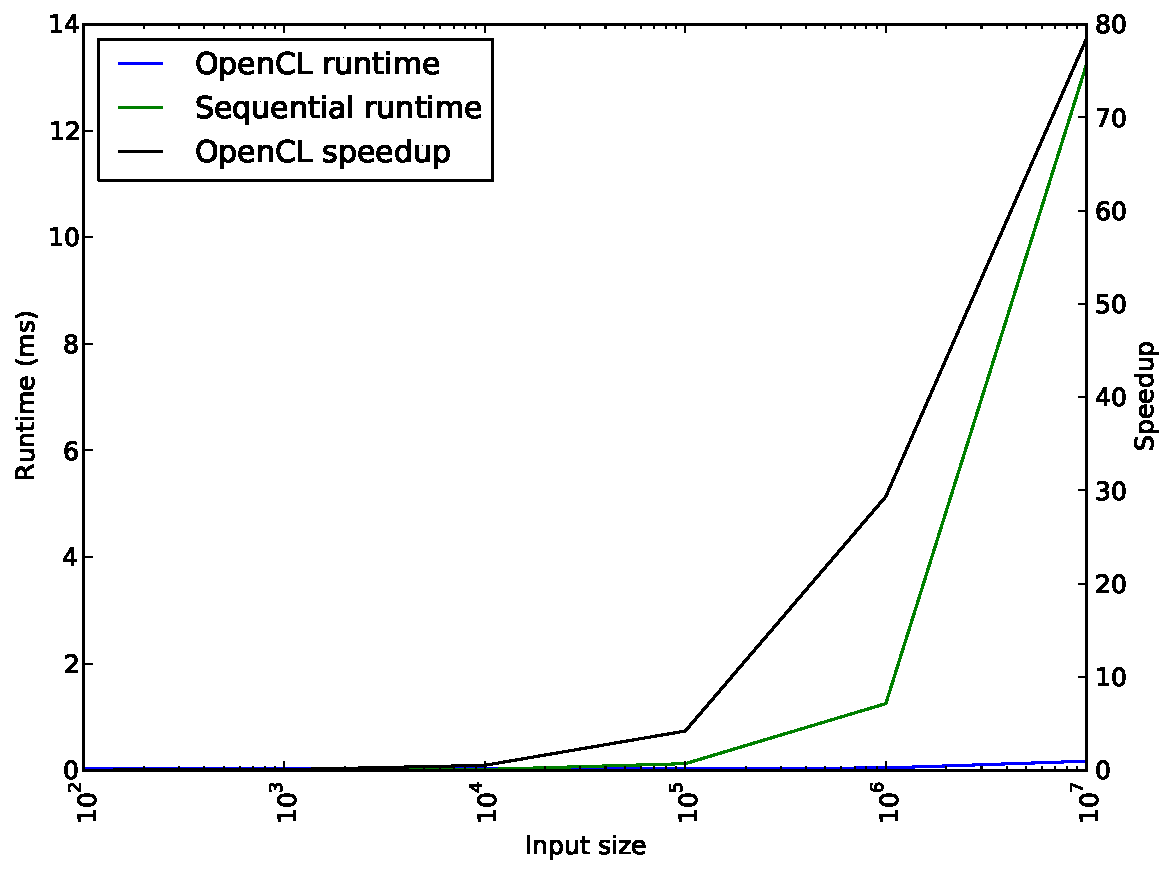
\includegraphics[width=0.8\textwidth]{test_process.pdf}
    \caption{benchmarks of \texttt{test\_process}}
\end{figure}

\begin{figure}
    \centering
    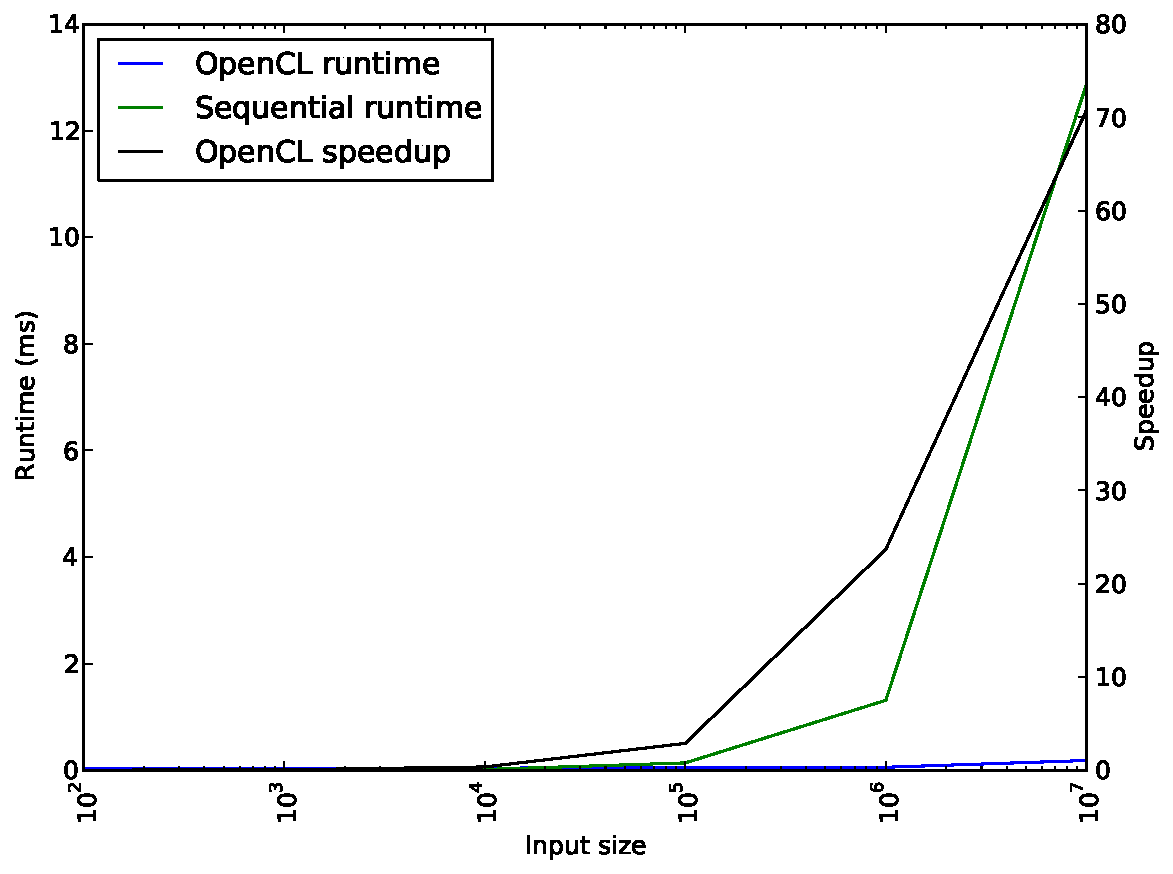
\includegraphics[width=0.8\textwidth]{test_process_idx.pdf}
    \caption{Benchmarks of \texttt{test\_process\_idx}}
\end{figure}

\FloatBarrier

\section*{Exercise 2}

The code for the Hillis-Steele prefix sum is given below.
For each step in the loop, it constructs new values for certain indices and uses
scatter to update \verb|xs| with these new values.

\begin{minted}{haskell}
def hillis_steele [n] (xs: [n]i32) : [n]i32 =
  let m = ilog2 n
  in loop xs = copy xs for d in 0...(m-1) do
    let k  = 2**d |> i64.i32
    let is = map (+k) (iota (n - k))
    let vs = map (\i -> xs[i] + xs[i-k]) is
    in scatter xs is vs
\end{minted}

The code for the work-efficient prefix sum is given below.
Like Hillis-Steele, it constructs a list of new values at certain indices and
uses \verb|scatter| to update \verb|xs|. This is done over both a "upsweep" and
"downsweep" step. In the downsweep step, two sets of value/indices pairs are
constructed (one for the blue and black arrows and one for the red arrows from
the slides).

\begin{minted}{haskell}
def work_efficient [n] (xs: [n] i32) : [n] i32 =
  let m = ilog2 n
  let upswept =
    loop xs = copy xs for d in (m-1)..(m-2)...0 do
      let k  = 2**d       |> i64.i32
      let k' = 2**(m-d-1) |> i64.i32
      let is = map (\i -> 2*i*k' + 2*k'-1) (iota k)
      let vs = map (\i -> xs[i]+xs[i-k']) is
      in scatter xs is vs
  let upswept[n-1] = 0
  let downswept =
    loop xs = upswept for d in 0...(m-1) do
      let k   = 2**d       |> i64.i32
      let k'  = 2**(m-d-1) |> i64.i32
      let is1 = map (\i -> 2*i*k' + 2*k'-1) (iota k)
      let is2 = map (\i -> 2*i*k' +   k'-1) (iota k)
      let vs1 = map (\i -> xs[i]+xs[i-k']) is1 -- Black & blue arrows
      let vs2 = map (\i -> xs[i+k'])       is2 -- Red arrows
      let k2  = k*2 -- Can't write expression in type cast
      let is  = is1 ++ is2 :> [k2]i64
      let vs  = vs1 ++ vs2 :> [k2]i32
      in scatter xs is vs
  in downswept
\end{minted}

Benchmarks comparing the Hillis-Steele, work-efficient and built-in scan is
shown below. The benchmarks were all on the \verb|gpu04-diku-apl| machine using
openCL. (the graph was plotted on my own machine as the ones generated on GPU04
looked weird).

\begin{figure}
    \centering
    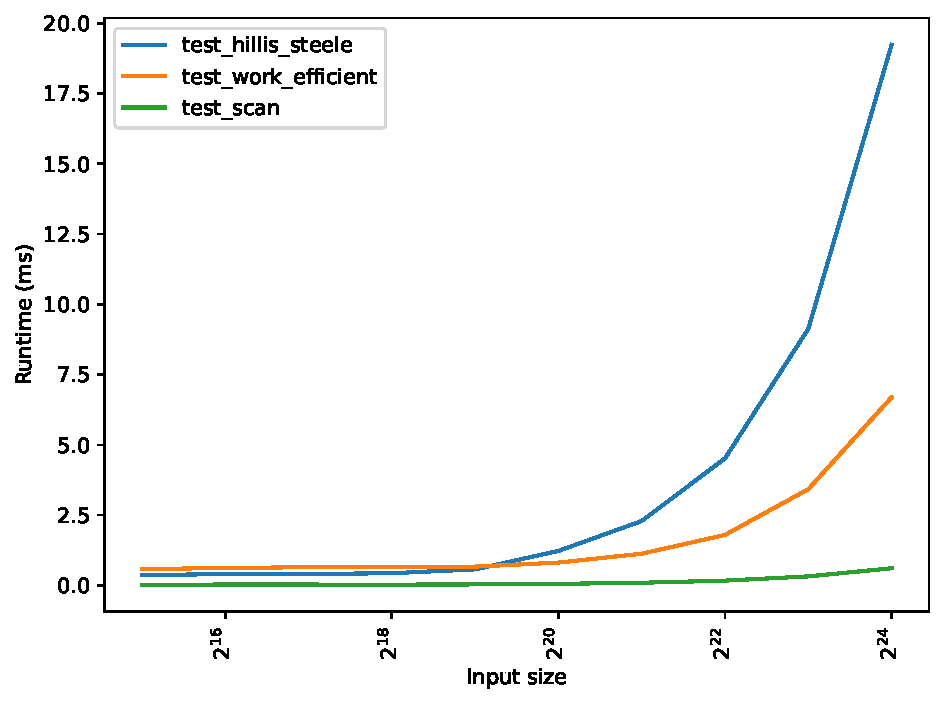
\includegraphics[width=0.8\textwidth]{prefix-sum.pdf}
    \caption{benchmarks of prefix sums}
\end{figure}

While it's not easy to eyeball from the graph if the Hillis-Steele algorithm
follows a $O( n \log n)$ curve it is clear that the runtime of the Hillis-Steele
algorithm grows faster than the runtime of the work-efficient algorithm as the
input size grows, which would suggest that the work-efficient algorithm has a
better asymptotic runtime (or at least better constants w.r.t scaling).

They are both, however, much slower than the built-in scan.


\section*{Exercise 3}

\subsection*{3.1}

In the definition of $\assoc'$ we substitute the values $f_1$ and $v_1$ with
\verb|0| and \verb|false| respectively:

\begin{align*}
     & \texttt{
        (if $f_2$ then $v_2$ else $0 \assoc v_2$, $\texttt{false} \conj f_2$)
    }
    \\
    \intertext{We use the fact that $0$ is the neutral element of $\assoc$.}
    =& \texttt{
        (if $f_2$ then $v_2$ else $v_2$, $\texttt{false} \conj f_2$)
    }
    \\
    \intertext{
        And the fact that \texttt{false} is the neutral element of $\conj$.
    }
    =& \texttt{
        (if $f_2$ then $v_2$ else $v_2$, $f_2$)
    }
    \\
    \intertext{
        Finally we get rid of the redundant if-statement.
    }
    =& \texttt{
        ($v_2$, $f_2$)
    }
    \\
\end{align*}

\subsection*{3.2}

The benchmarks of segmented scan and reduce are shown below, compared with
normal scan and reduce. The benchmarks were done on the \verb|gpu04-diku-apl| machine
using openCL. The segmented scan/reduce were with addition over a random array
with a random boolean flag array meaning the average segment length is very short
compared to what you would expect from a realistic workload, which might impact
the preformance.

\begin{figure}
    \centering
    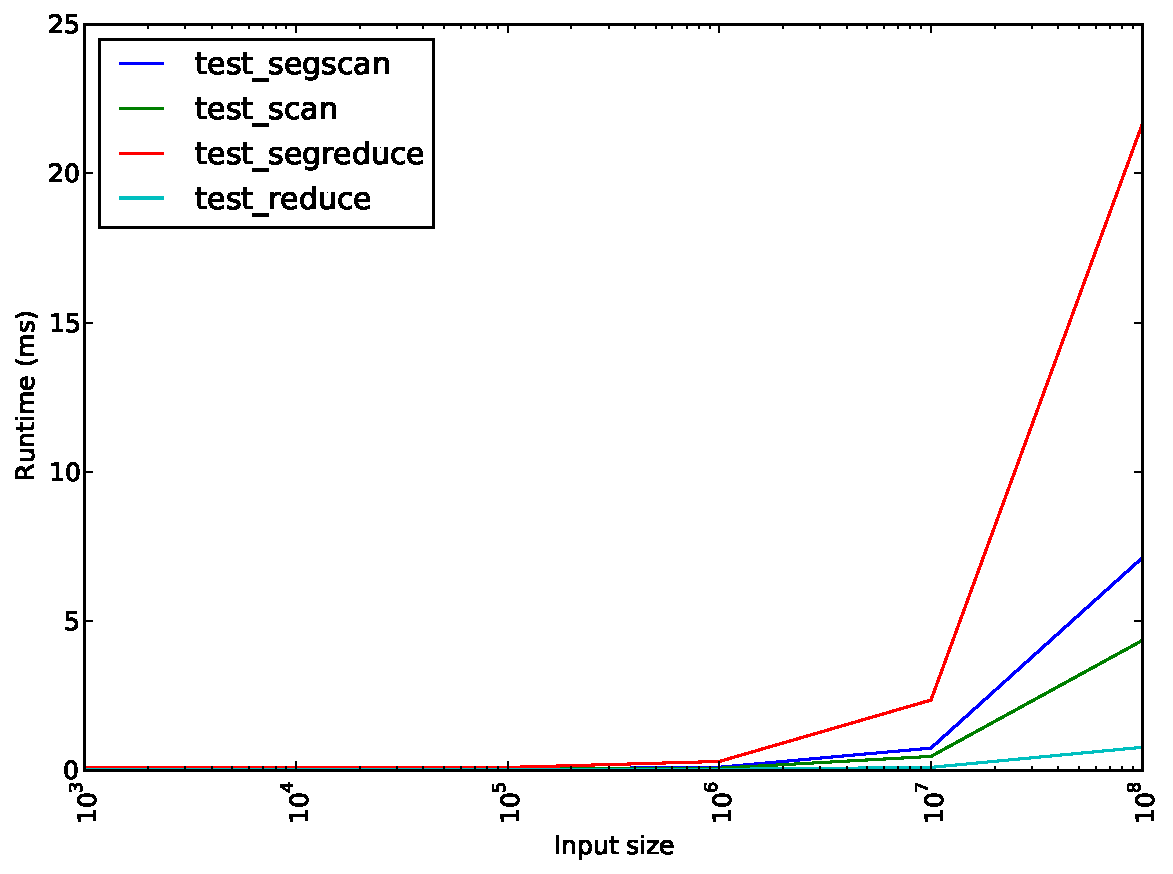
\includegraphics[width=0.8\textwidth]{segmented.pdf}
    \caption{Benchmarks of segmented scan and reduce}
\end{figure}

As can be seen from the benchmarks, segmented scan is only a little slower than
normal scan, which is to be expected from the more complicated operator.
Segmented reduce is much slower than normal reduce as segmented reduce is built
on top of segmented scan with additional bookkeeping to collect the results.

\end{document}
